%%%% Paramétrage du TD %%%%
\def\xxactivite{ \ifprof \normalsize{Application 1 -- Corrigé } \else  \ifcolle Colle \else Application 1\fi \fi} % \normalsize \vspace{-.4cm}
\def\xxauteur{\textsl{Xavier Pessoles}}


\def\xxnumchapitre{Chapitre 1 \vspace{.2cm}}
\def\xxchapitre{\hspace{.12cm} Détermination des liaisons équivalentes}


\def\xxcompetences{%
\textsl{%
\textbf{Savoirs et compétences :}\\
\begin{itemize}[label=\ding{112},font=\color{ocre}] 
\item B2-15 : Simplifier un modèle de mécanisme.
%\item \textit{Mod2.C34} : degré de mobilité du modèle;
%\item \textit{Mod2.C34} : degré d’hyperstatisme du modèle;
%\item \textit{Mod2.C34.SF1} : déterminer les conditions géométriques associées à l’hyperstatisme;
%\item \textit{Mod2.C34} : résoudre le système associé à la fermeture cinématique et en déduire le degré de mobilité et d’hyperstatisme.
\end{itemize}
}}


\def\xxtitreexo{Application 01}
\def\xxsourceexo{\hspace{.2cm} \footnotesize{P. Dupas}}


\def\xxfigures{
%\includegraphics[width=.7\linewidth]{axe_y_photo}
}%figues de la page de garde


\input{\repRel/Style/pagegarde_TD}
\setcounter{numques}{0}
\setlength{\columnseprule}{.1pt}
\pagestyle{fancy}
\thispagestyle{plain}
\vspace{5.2cm}

\def\columnseprulecolor{\color{ocre}}
\setlength{\columnseprule}{0.4pt} 


%%%%%%%%%%%%%%%%%%%%%%%

\setcounter{exo}{0}


\ifprof
\begin{multicols}{2}
\else
\begin{multicols}{2}
\fi


\subsection*{Liaisons en parallèle}

\question{Déterminer la liaison équivalente des liaisons suivantes.}

\begin{center}
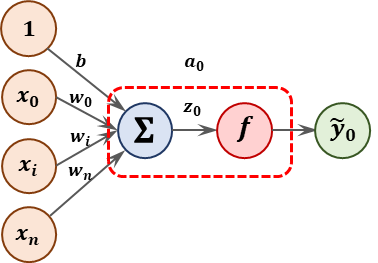
\includegraphics[width=.8\linewidth]{fig_01.png}
\end{center}

\begin{center}
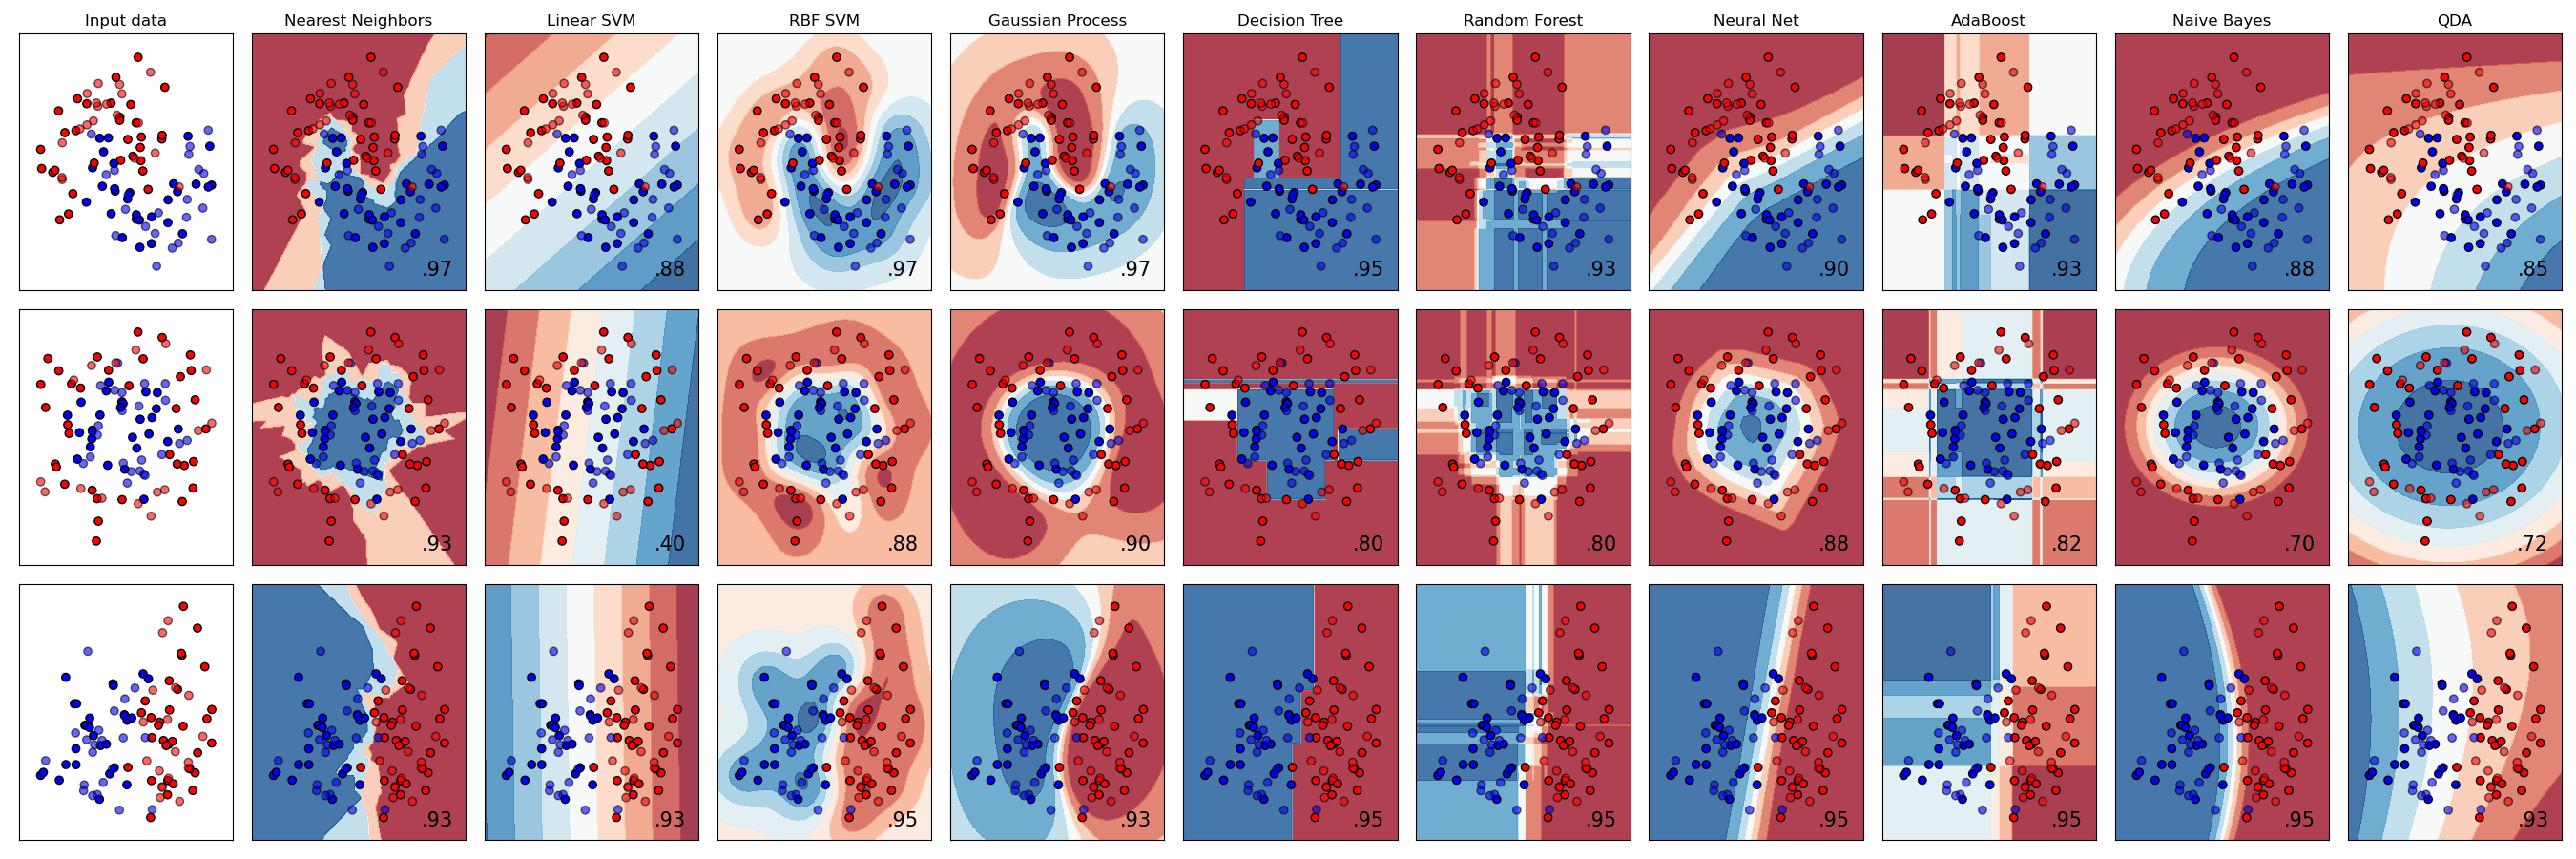
\includegraphics[width=.8\linewidth]{fig_02.png}
\end{center}

\begin{center}
\rotatebox{90}{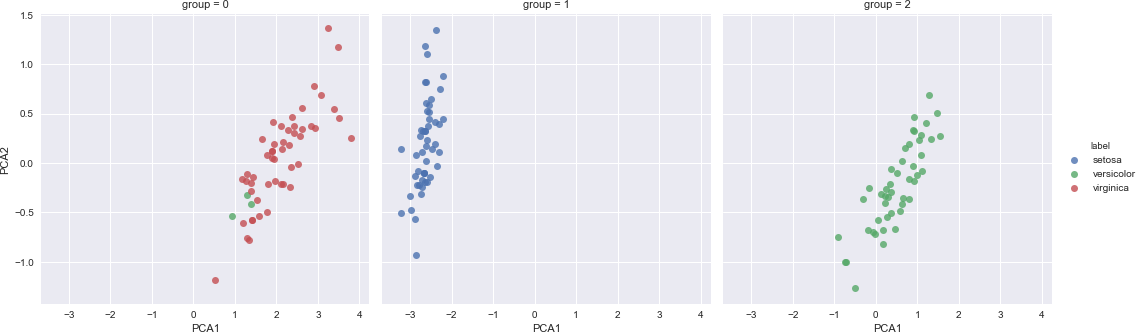
\includegraphics[width=.6\linewidth]{fig_03.png}}
\end{center}

\begin{center}
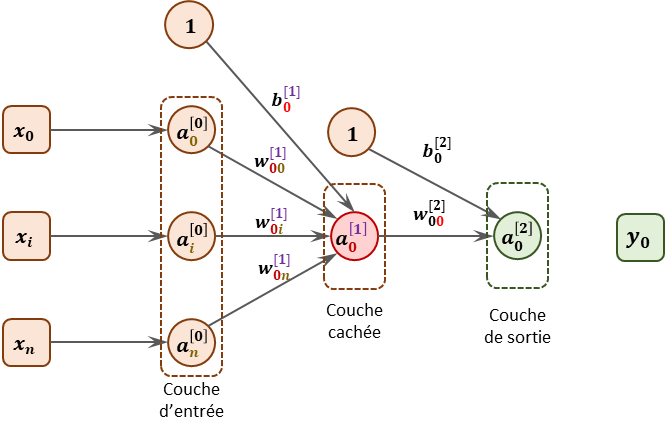
\includegraphics[width=.8\linewidth]{fig_04.png}
\end{center}

\begin{center}
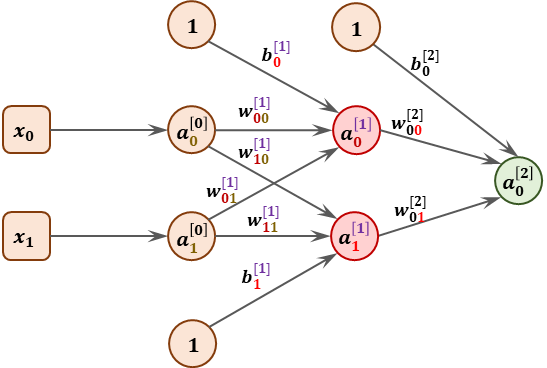
\includegraphics[width=.8\linewidth]{fig_05.png}
\end{center}

\begin{center}
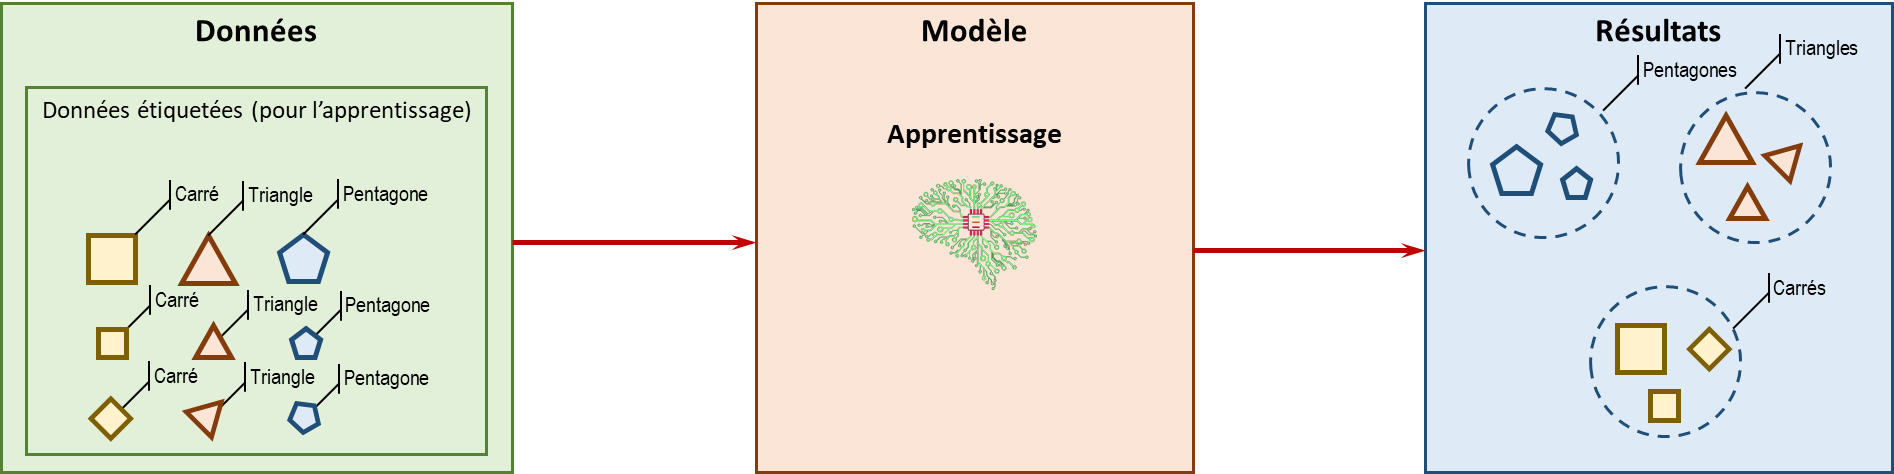
\includegraphics[width=.8\linewidth]{fig_06.png}
\end{center}

\begin{center}
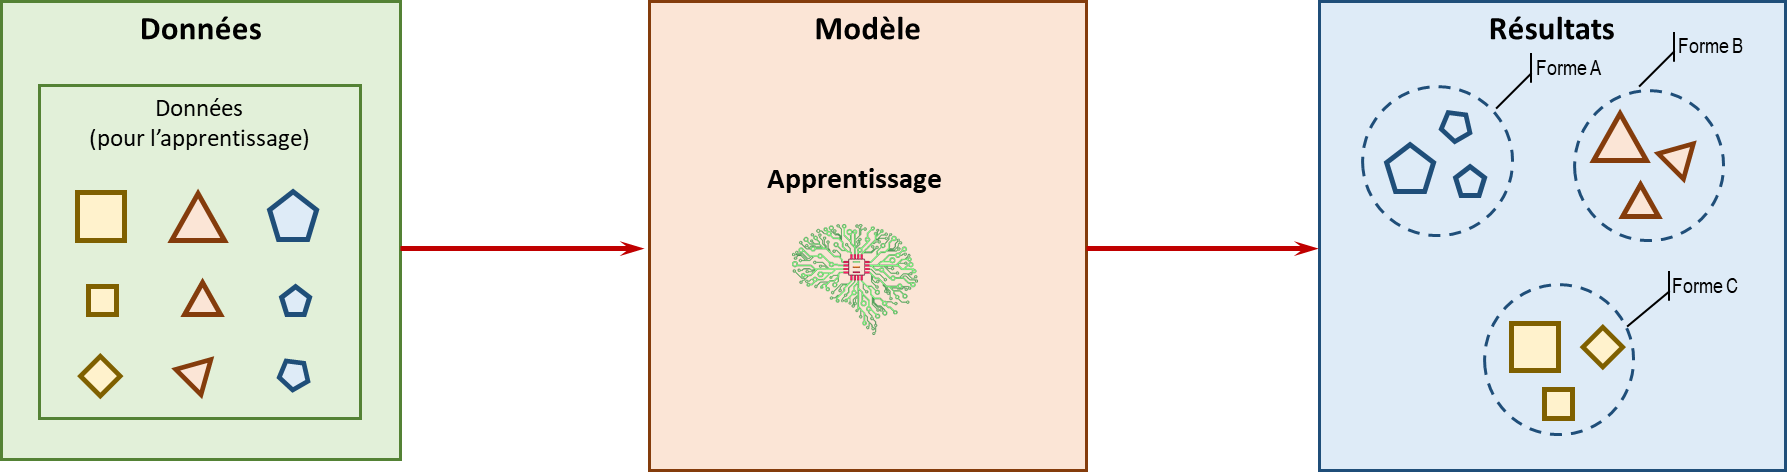
\includegraphics[width=.8\linewidth]{fig_07.png}
\end{center}

\begin{center}
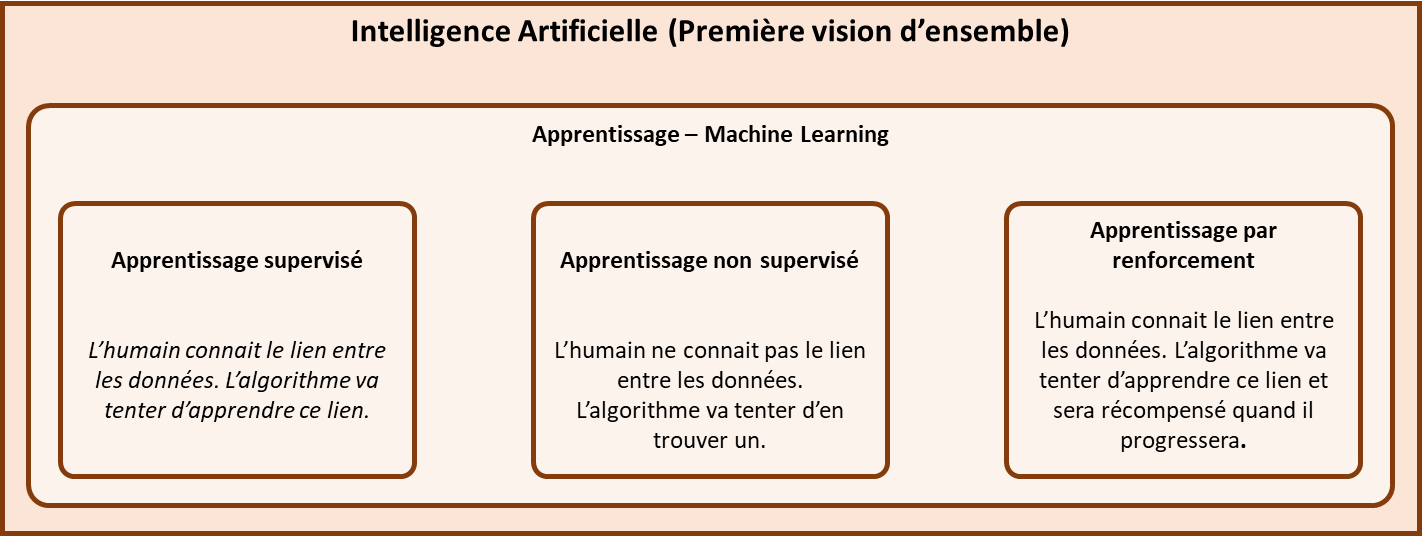
\includegraphics[width=.8\linewidth]{fig_08.png}
\end{center}

\begin{center}
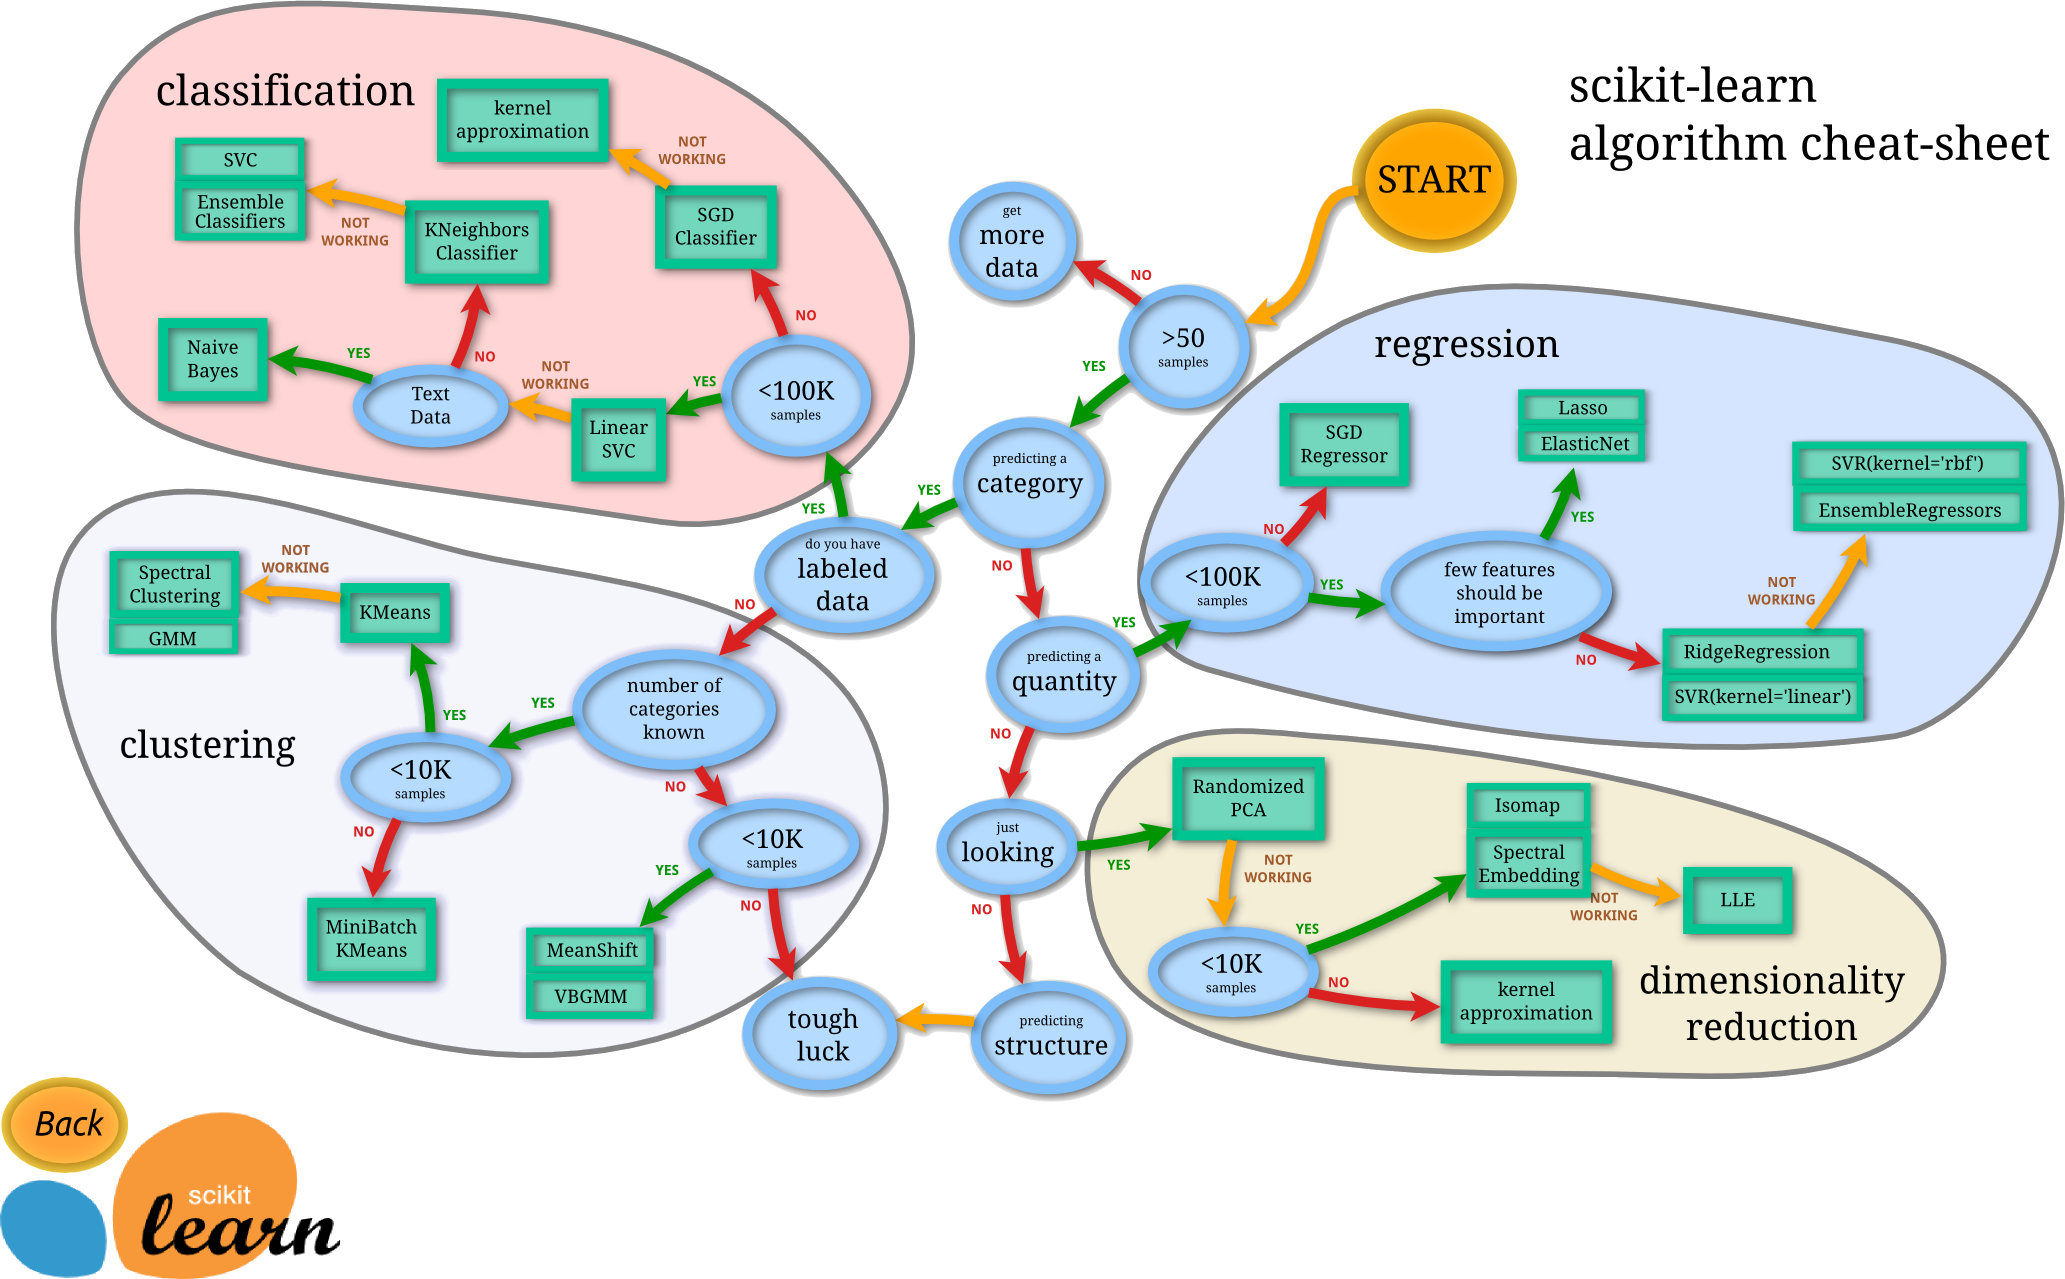
\includegraphics[width=.5\linewidth]{fig_09.png}
\end{center}

\begin{center}
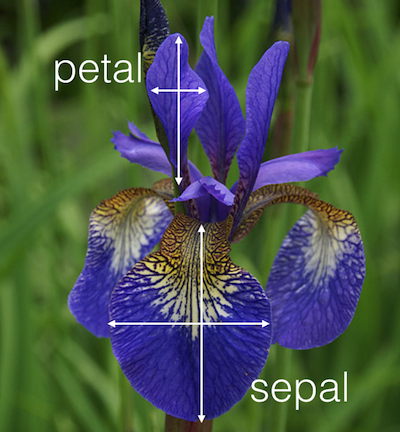
\includegraphics[width=.8\linewidth]{fig_10.png}
\end{center}


\subsection*{Liaisons en série}

\question{Déterminer la liaison équivalente des liaisons suivantes.}


\begin{center}
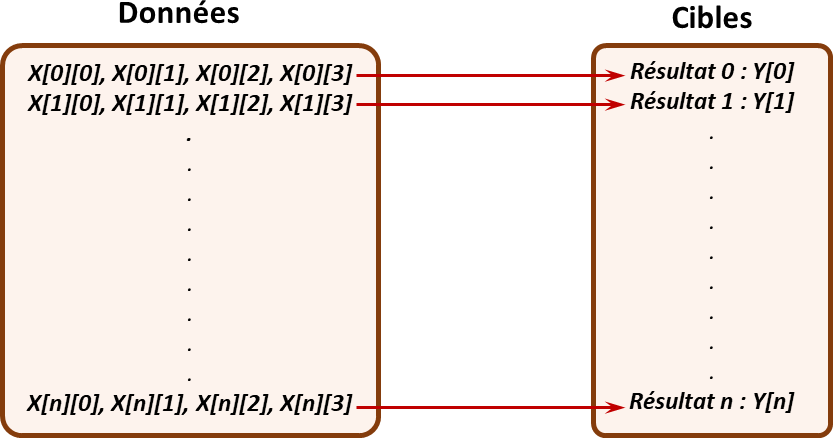
\includegraphics[width=.3\linewidth]{fig_11.png}
\hspace{1cm}
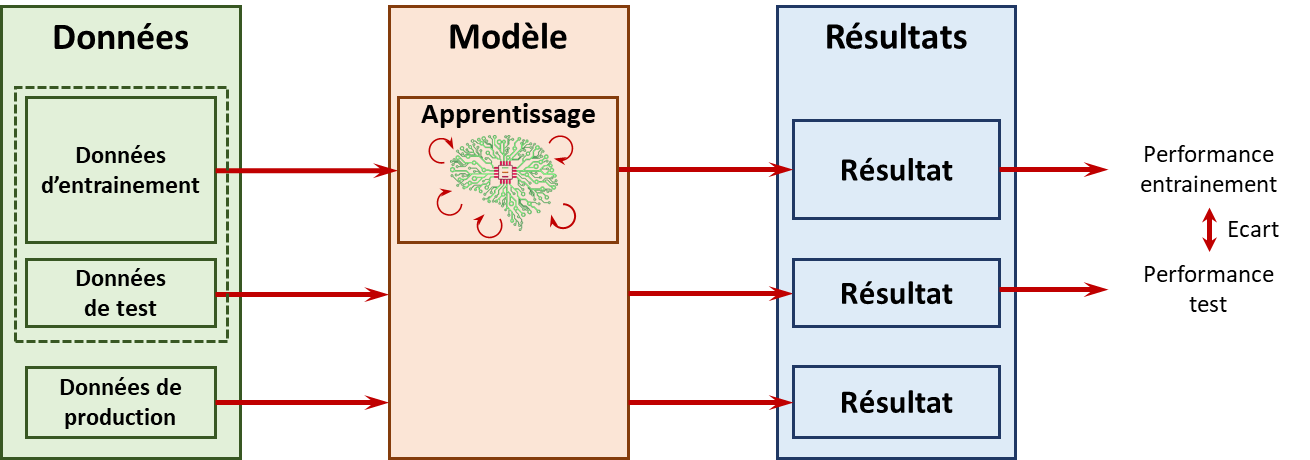
\includegraphics[width=.25\linewidth]{fig_12.png}
\end{center}

\ifprof
\end{multicols}
\else
\end{multicols}
\fi


